\documentclass{article}
\usepackage[magyar]{babel}
\usepackage{t1enc}
\usepackage{lipsum}
\usepackage{hulipsum}
\usepackage{tikz}
\usetikzlibrary{patterns}
\usetikzlibrary{shapes} 


\begin{document}

\tikz{ \draw (0,0) -- (1,0) -- (1,1) -- ++(120:1) -- (0,1) -- (0,0) -- (1,1) -- (0,1) -- (1,0) ; }

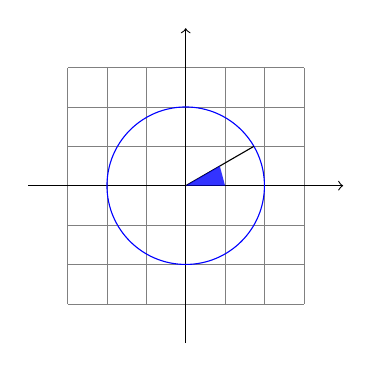
\begin{tikzpicture}
\draw[help lines, step=0.5]
(-1.5,-1.5) grid (1.5,1.5) ;
\draw[->] (-2,0) -- (2,0);
\draw[->] (0,-2) -- (0,2);
\draw[color=blue] circle [radius=1] ;
\draw (0,0) -- (30:1);
\fill[blue, opacity=0.8] (0,0) -- (0.5,0) -- (30:0.5);
\end{tikzpicture}

\tikz{ \fill[blue] (0,0) circle (2);
\filldraw[draw=yellow,fill=yellow,opacity=0.8,
fill opacity=0.8] (1,0) circle (2); }

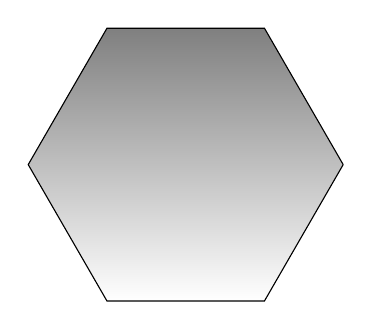
\begin{tikzpicture}

   \newdimen\R
\R=2cm
   \filldraw[draw=black, fill=black, shading=axis] (0:\R)
   \foreach \x in {60,120,...,360} {  -- (\x:\R) }
 ;
\end{tikzpicture}

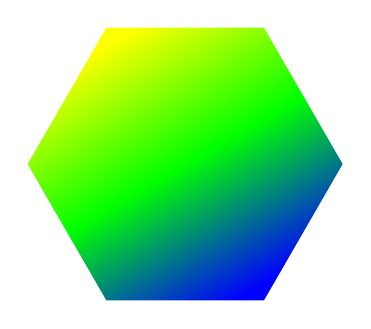
\begin{tikzpicture}
\newdimen\R
\R=2cm
\shade[top color=yellow, bottom color=blue,
middle color=green, shading angle=30]
(0:\R)
   \foreach \x in {60,120,...,360} {  -- (\x:\R) };
\end{tikzpicture}


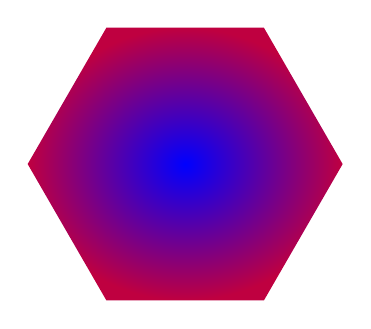
\begin{tikzpicture}
\newdimen\R
\R=2cm
\shade[shading=radial, outer color=purple,
inner color=blue]
(0:\R)
   \foreach \x in {60,120,...,360} {  -- (\x:\R) };
\end{tikzpicture}


\begin{tikzpicture}
\newdimen\R
\R=4cm
\newcommand{\utvonalam}{(0,0) -- ++(45:1) -- ++(135:1) -- ++(225:1) -- (0,0);}
\fill[purple] \utvonalam ;
\pattern[pattern=sixpointed stars,
pattern color=yellow] \utvonalam ;
\end{tikzpicture}

\tikz{\shade[shading=ball, ball color=purple]
(0,0) circle (2);}

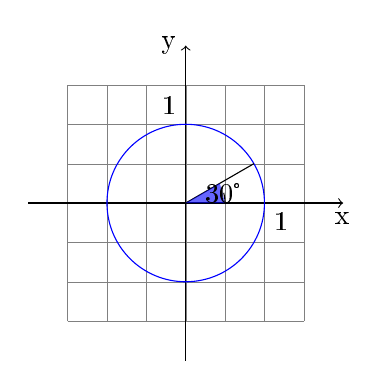
\begin{tikzpicture}
\draw[help lines, ultra thin, step=0.5]
(-1.5,-1.5) grid (1.5,1.5) ;
\draw[->] (-2,0) -- (2,0) node[below] {x};
\draw[->] (0,-2) -- (0,2) node[left] {y};
\draw[color=blue] circle [radius=1] ;
\draw (0,0) -- (30:1);
\fill[blue, opacity=0.6] (0,0) -- (0.5,0) -- (30:0.5);
\draw (0.5,0) arc (0:15:0.5) node{30°};
\draw (1,0) node [below right] {1} (0,1) node[above left] {1};
\end{tikzpicture}

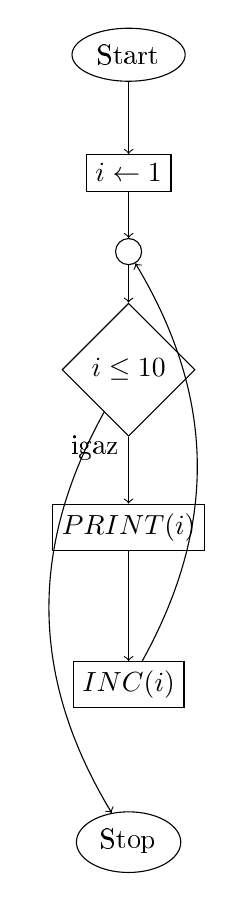
\begin{tikzpicture}
\path (0,0) node[ellipse,draw](Start) {Start}
(0,-1.5) node[rectangle,draw](i_1) {$i \leftarrow 1$}
(0,-2.5) node[circle,draw](c) {}
(0, -4) node[diamond,draw](i_10) {$i \leq 10$}
(0, -6) node[rectangle,draw](i_print) {$PRINT(i)$}
(0, -8) node[rectangle,draw](i_inc) {$INC(i)$}
(0,-10) node[ellipse,draw](Stop) {Stop}
;
\draw[->] (Start) -- (i_1);
\draw[->] (i_1) -- (c);
\draw[->] (c) -- (i_10);
\draw[->] (i_10) -- (i_print);
\draw (i_10) -- (0,-5) node[left] {igaz};
\draw[->] (i_print) -- (i_inc);

\draw (i_inc) edge[->,bend right] (c);
\draw (i_10) edge[->,bend right] (Stop);

\end{tikzpicture}



\end{document}